\chapter{Interaction Region Local Coupling Correction in the LHC} % Main chapter title
\label{chapter:IR_Local_Coupling} % For referencing the chapter elsewhere, use \cref{chapter:IR_Local_Coupling}

Some paragraph before the first section. Blah.

%----------------------------------------------------------------------------------------

\section{Local Betatron Coupling in the Interaction Regions}

\textbf{List of things to include in this section:}
\begin{itemize}
    \item Equivalency of Ripken and Tracking when looking at beam size (or later?)
    \item ALICE \num{2018} ion run lumi issue
    \item Projection of the beam size growth and lumi in the LHC vs HL-LHC
    \item Include the parts in the "relevant theory" section of my PRAB paper
    \item Refer to previous chapter plots of IR for the very large \(\beta\)-functions in the triplet quadrupoles, tilts in these magnets have the potential to drastically contribute to the magnitude of the \(f_{1001}\) term, and therefore to the coupling in the interaction region and, if not compensated properly, to the coupling in the whole machine
\end{itemize}

\begin{equation}
    \langle z \rangle = \sqrt{\varepsilon_1 \beta_{1z} + \varepsilon_2 \beta_{2z}}, \quad z \in\{x, y\} ,
    \label{equation:lebedev_beam_size}
\end{equation}
where \(\varepsilon_1\) and \(\varepsilon_2\) are the horizontal and vertical emittances, respectively.
\Cref{figure:ip_ellipses_from_coupling} shows a reconstruction of transverse beam sizes at IP\num{5} under varying strength of a local coupling bump.
While the beam ellipses show a \(\gg\) \qty{99}{\percent} overlap indicating a negligible tilt effect, the beam size in the most affected case is about \qty{250}{\percent} of the uncoupled case.

\begin{figure}[!htb]
    \centering
    \includegraphics*[width=0.75\columnwidth]{Figures/IR_Coupling_Correction/ellipses_various_coupling_bumps.pdf}
    \caption{Transverse beam sizes at IP\num{5} at \qty{6.8}{\tera\electronvolt} and \(\beta^{\ast}=\)~\qty{30}{\centi\meter} with normalized emittances \(\varepsilon_x = \varepsilon_y =\)~\qty{3.75}{\micro\meter} and for different strengths of a local coupling bump around the IP. The ellipses are reconstructed through the \(\sigma_{11}\), \(\sigma_{13}\) and \(\sigma_{33}\) terms of the sigma matrix, obtained from MAD-X.}
    \label{figure:ip_ellipses_from_coupling}
\end{figure}

Instantaneous luminosities calculated for~\cref{figure:lhc_vs_hllhc_beam_size_and_lumi_growths}, in the absence of crossing angles, are done so according to~\cite{CERN:Herr:Concept_Luminosity}:

\begin{equation}
    \mathcal{L} = \frac{N_1 N_2 f_{rev} N_b}{2 \pi \sqrt{\left( \sigma_{x, 1}^2 + \sigma_{x, 2}^2 \right)} \sqrt{\left( \sigma_{y, 1}^2 + \sigma_{y, 2}^2 \right)}} ,
    \label{equation:luminosity_double_beams}
\end{equation}
where \(N_{n}\) is the number of protons per bunch in beam \(n\), \(f_{rev}\) the revolution frequency of particles, \(N_b\) the number of bunches per beam and \(\sigma_{z, n}\) is the size at the IP of beam \(n\) in the transverse plane \(z\), calculated according to \cref{equation:lebedev_beam_size}.

\begin{figure}[!htb]
    \centering
    \includegraphics*[width=0.99\columnwidth]{Figures/IR_Coupling_Correction/lhc_vs_hllhc_combined.pdf}
    \caption{Relative values of the RMS beam size at IP\num{1} (\textcolor{mplblue}{blue}) as well as luminosity (\textcolor{mplorange}{orange}) for different strengths of a local coupling bump around the IP made with skew quadrupoles, for the LHC (filled) and HL-LHC V1.5 (dashed). Beam sizes are calculated according to \cref{equation:lebedev_beam_size} and luminosities according to \cref{equation:luminosity_double_beams}. In the case of the HL-LHC, the relative beam size increase and subsequent luminosity loss are greater due to the larger \(\beta\)-functions in the triplet.}
    \label{fig:lhc_vs_hllhc_beam_size_and_lumi_growths}
\end{figure}

\section{Current Correction Methods and Their Limitations}

Overview of IR Difficulties (phase advances suck, DFFT of x -jpx, no instruments, SbS errors)

In the LHC, a skew quadrupole corrector is installed on each side of colliding IPs, just before the third triplet quadrupole \(\mathrm{Q3}\) on the side of the IP.
Due to their location, these correctors are single aperture magnets meaning that both beams are passing through a single cavity, and feel the same magnetic field.
As the triplet quadrupoles - also single aperture magnets - are expected to be most of the contribution to local coupling, the local error to be corrected should be the same for both beams and such an arrangement of correctors is manageable.

Say that looking at RDTs is just not straightforward, and give example with plot below. Can you guess who's better? I forgot already.
\begin{figure}
    \centering
    \includegraphics*[width=0.99\linewidth]{Figures/IR_Coupling_Correction/similar_rdts_different_ip1_lumi.pdf}
    \caption{Similarly looking coupling RDTs from two measurements (top and bottom) in the LHC \num{2022} commissioning. One scenario leads to a \qty{20}{\percent} luminosity decrease at IP\num{1} compared to the other. Can you tell which is which?}
    \label{figure:guess_rdts}
\end{figure}

\begin{table}[!hbt]
    \centering
    \begin{tblr}{colspec={ccccc}}
        \hline
        \textbf{Magnet} & \textbf{K\(_{1S}\) [m\(^{-2}\)]}    \\
        \hline
        MQSX.3R[IP] \(\rightarrow K_{1S}\)  &  \num{1E-4}   \\
        MQSX.3L[IP] \(\rightarrow K_{1S}\)  &  \num{-1E-4}  \\
        \hline
    \end{tblr}
    \caption{Definition of one unit of the colinearity knob, a powering setting of the IR skew quadrupole correctors.}
    \label{table:colin_knob}
\end{table}

\begin{figure}
    \centering
    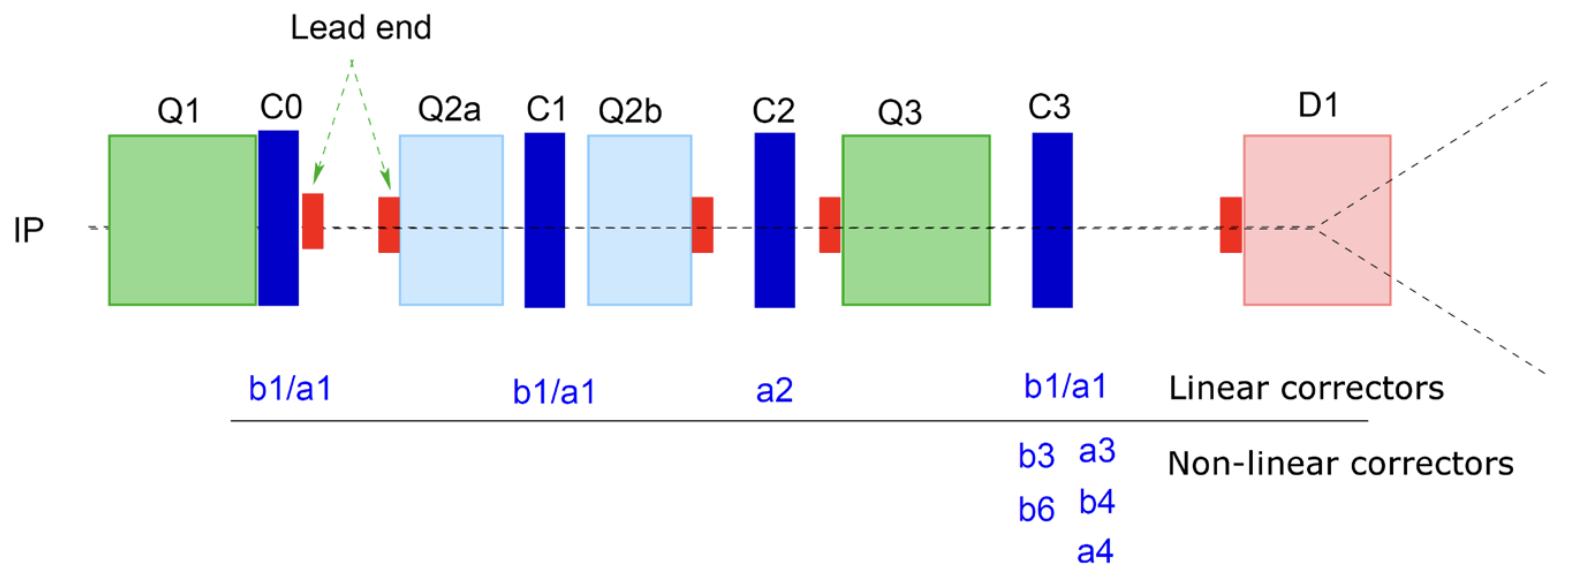
\includegraphics[width=0.9\linewidth]{Figures/IR_Coupling_Correction/corrector_package.png}
    \caption{Layout of the triplet magnets and the linear and nonlinear correctors in the LHC experimental insertions~\cite{CERN:Bruning:Dynap_Studies}, showing common aperture magnets. The Q\num{1}, Q\num{2}a/b and Q\num{3} are triplet quadrupoles while the C\num{0}, C\num{1}, C\num{2} and C\num{3} are corrector packages with the field order indicated below. D\num{1} is the separation dipole, diverging Beam \num{1} and Beam \num{2} to their respective beam lines. The skew quadrupole correctors correspond to order a\num{2} and are located in the C\num{2} package.}
    \label{figure:lhc_corrector_layout}
\end{figure}

\todo{Here include also the stuff that didn't work (CRDTs, k-modulation, etc.)}

\section{Rigid Waist Shift for Local Coupling Correction}

\subsection{Concept and Simulations}

\begin{figure}
    \centering
    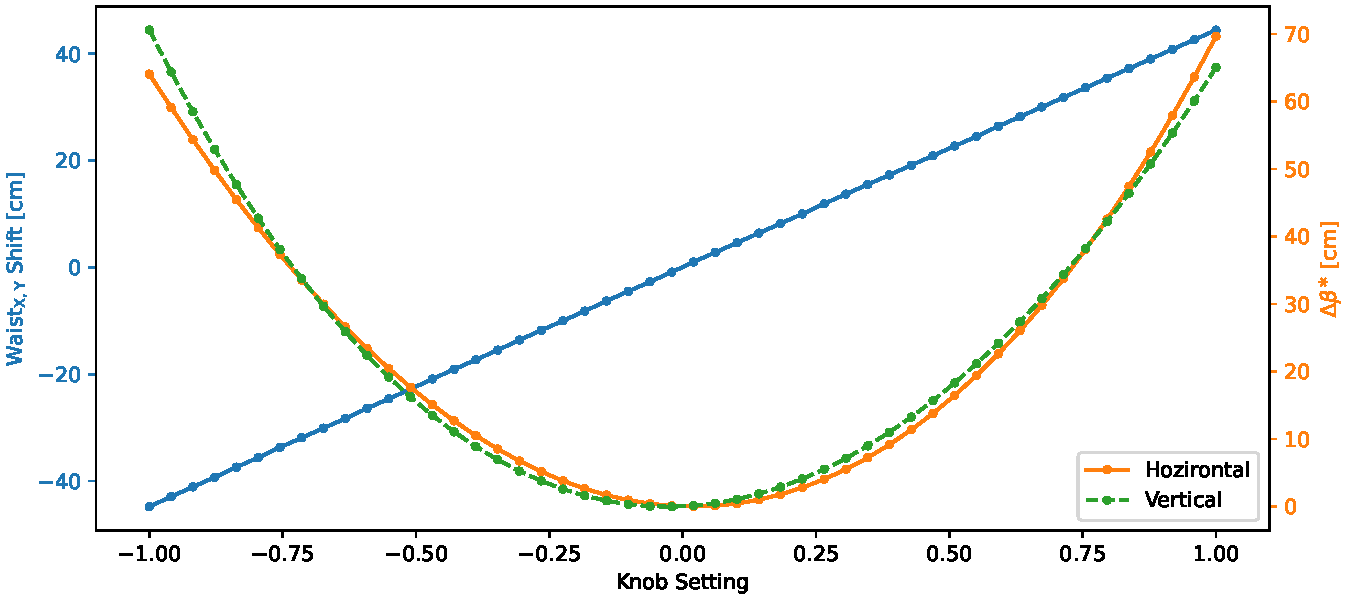
\includegraphics[width=0.9\textwidth]{Figures/IR_Coupling_Correction/rigid_waist_shift_effect_combined.pdf}
    \caption{Simulated effect of the designed rigid waist shift knob on the \(\beta^{\ast} =\) \qty{30}{\centi\metre} collision optics. The \textcolor{mplblue}{blue} line represents the waist displacement from the design location and is almost completely linear with the knob setting. The \textcolor{mplorange}{orange} and \textcolor{mplgreen}{green} lines represent the horizontal and vertical \(\beta\)-functions change at the IP point itself as the waist is displaced, respectively. The minima of the parabolas are not found at the zero knob setting as the design optics include a very small waist.}
    \label{figure:rigid_waist_shift_knob_effect1}
\end{figure}

\begin{figure}[!htb]
    \centering
    \includegraphics*[width=\columnwidth]{Figures/IR_Coupling_Correction/waist_shift_leaks_rdts.pdf}
    \caption{Linear coupling RDTs in the vicinity of IP\num{1} under a coupling bump, with (\textcolor{mplr}{red}) and without (\textcolor{mplb}{blue}) an RWS. The vertical \textcolor{mqsx_green}{green} lines represent the positions of the skew quadrupoles correctors (MQSX.\num{3}[RL]\num{1}) used to implement the coupling bump. A colinearity knob setting of \num{10} and a rigidity waist shift knob setting of \num{1} were used, which results in a \qty{0.5}{\percent} change in the triplet powering knob and a \qty{43.5}{\centi\meter} shift of the beam waists.}
    \label{figure:rdt_leak}
\end{figure}

\begin{figure}[!htb]
    \centering
    \includegraphics*[width=0.99\columnwidth]{Figures/IR_Coupling_Correction/colin_knob_vs_waist_shift.pdf}
    \caption{Impact of the colinearity knob on the global \(\abs{C^{-}}\), calculated according to \cref{equation:deltaqmin_from_f1001}, with and without applying an RWS.}
    \label{figure:knob_to_cminus_with_waist}
\end{figure}

\Cref{figure:cminus_colin_vs_tilt_with_waist} shows the values of the resulting \(\abs{C^{-}}\) across the parameter space when an RWS is applied.

\begin{figure}[!htb]
    \centering
    \includegraphics*[width=0.99\columnwidth]{Figures/IR_Coupling_Correction/cminus_colin_tilt_compensation_with_waist.pdf}
    \caption{Resulting \(\abs{C^{-}}\) (\cref{equation:deltaqmin_from_f1001}) for various combinations of tilt error and colinearity knob settings, when applying an RWS.}
    \label{figure:cminus_colin_vs_tilt_with_waist}
\end{figure}

\Cref{figure:beam_size_colin_vs_tilt_no_waist} shows the resulting beam size increase as a ratio to the nominal beam size across the same parameter space, highlighting that minimization of the growth is possible though a wrong setting would enhance the phenomenon.

\begin{figure}[!htb]
    \centering
    \includegraphics*[width=0.99\columnwidth]{Figures/IR_Coupling_Correction/ip_beam_size_growth_colin_tilt_compensation_no_waist.pdf}
    \caption{Resulting beam size (\cref{equation:lebedev_beam_size}) increase for identical settings of tilt error and colinearity knob settings as \cref{figure:cminus_colin_vs_tilt_with_waist}, but without an RWS.}
    \label{figure:beam_size_colin_vs_tilt_no_waist}
\end{figure}

\subsection{Determining Corrections}

Blah.

%----------------------------------------------------------------------------------------

\section{Experimental Results from the LHC \num{2022} Commissioning}

Can refer to appendix \Cref{appendix:experimental_knobs} for the fills used.

\begin{table}[!htb]
    \centering
    \caption{Luminosity gains observed at the main experiments ATLAS and CMS from the method's suggested corrections.}
    \begin{tblr}{colspec={ccc}}
        \hline
        \SetCell[r=2,c=1]{m,c} \textbf{Experiment} & \SetCell[c=2]{c} \textbf{Luminosity Gain [\unit{\percent}]}                     \\
        \cline{2,3}                                &    \(\beta^{\ast} = \) \qty{30}{cm}    &    \(\beta^{\ast} = \) \qty{42}{cm}    \\
        \hline
        \textbf{ATLAS (IP\num{1})}                 &    \num{9.7}                           &     \num{5.2}                          \\
        \textbf{CMS (IP\num{5})}                   &    \num{3.5}                           &     \num{1.5}                          \\
        \hline
    \end{tblr}
    \label{table:rws_lumi_gains}
\end{table}

\section{Operation with Limited Correctors Availability}

Mitigation Options in Case of MQSX Failures

(A lot here should be taken from my project update V talk at the QUASAR group.)

\subsection{Lifetime Considerations of MQSX Elements}

Explain that there is a real risk that some of our MQSX magnets die, especially the ones in IR1 (ATLAS).
In this case, we will need a containment plan, as not only are they used for the but the local corrections they are a part of are a baseline for us to compute higher order terms corrections.

\Cref{table:correctors_peak_dose} reproduced from slide 23~\cite{Evian21:Cerutti:TripletLifetime}:

\begin{table}[!htb]
    \centering
    \caption{Expected total received dose of the corrector magnets located in the triplets for the main IRs. Table reproduced from~\cite{Evian21:Cerutti:TripletLifetime}. The entries marked with \asterisk assume an IR\num{1} polarity inversion in the middle of \num{2025}.}
    \begin{tblr}{colspec={ccc}}
        \hline
        \SetCell[r=3,c=1]{m,c} \textbf{Magnets}             &  \SetCell[c=2]{c} \textbf{Peak Dose [\unit{\mega\gray}]}                                                                                     \\
        \cline{2,3}                                         &  With ATLAS Variable (Fixed) Angle                        &    +\num{2025} (as \num{2023}/\num{2024})                                        \\
        \cline{2,3}                                         &  After \qty{395}{\femto\barn^{-1}}                        &    After \qty{480}{\femto\barn^{-1}}                                             \\
        \hline
        \textcolor{red}{\textbf{MCBX\num{1} (IR\num{1})}}   &    \textcolor{red}{\num{8.5} (\num{8.5})}                 &     \textcolor{red}{\num{11} (\num{11}) $/$ \asterisk \num{10.5} (\num{10.5})}   \\
        \textcolor{red}{\textbf{MCBX\num{1} (IR\num{5})}}   &    \num{6}                                                &     \textcolor{red}{\num{7.5}}                                                   \\
        \textbf{MCBX\num{2} (IR\num{1})}                    &    \num{3.5} (\num{3.5})                                  &     \num{4} (\num{4}) $/$ \asterisk \num{4} (\num{4})                            \\
        \textbf{MCBX\num{2} (IR\num{5})}                    &    \num{2}                                                &     \num{2.5}                                                                    \\
        \textcolor{red}{\textbf{MQSX (IR\num{1})}}          &    \textcolor{red}{\num{7.5} (\num{7.5})}                 &     \textcolor{red}{\num{9} (\num{9}) $/$ \asterisk \num{9} (\num{9})}           \\
        \textcolor{red}{\textbf{MQSX (IR\num{5})}}          &    \textcolor{red}{\num{8} (\num{8})}                     &     \textcolor{red}{\num{9.5} (\num{9.5})}                                       \\
        \textbf{MCBX\num{3} (IR\num{1})}                    &    \num{5} (\num{5})                                      &     \num{6} (\num{6.5}) $/$ \asterisk \num{6} (\num{6})                          \\
        \textbf{MCBX\num{3} (IR\num{5})}                    &    \num{3}                                                &     \num{3.5}                                                                    \\
        \hline
    \end{tblr}
    \label{table:correctors_peak_dose}
\end{table}

\todo{Important quote from the end of the presentation:}
"Assuming a limit of \qty{6}{\mega\gray} for the corrector magnets in the triplet, this is expected to be reached in the four \(\mathrm{MCBX.1}\) and four \MQSX by the end of \num{2024}."

This means in simple terms that MQSX dying will drastically impact the LHC's operations, and potentially shut the machine down.

\subsection{Tilt of Triplet Elements}

Talk about what we want to do (tilt Q3 or Q2) to induce a skew component + simulation results.
Found settings of the Q3 or Q2 that would negate the MQSX one determined in beam test / commissioning.
Show some plots, and come up with the tilt values that would be needed to do the compensation.

Also show we have a very minimal beta-beating from this.
Show we have had a look at different optics (30cm and 1m betastar) and it works for both.

\subsubsection{Operational Constraints}

The LHC systems are not meant for this, but for vertical alignment of these magnets!
System relies on bellows: 2 pieds IP side and 1 pied other side for Q2 for instance.
This means that inducing rotation is not only not the design purpose, but also imperfect (on move les 2 pieds pour essayer de mimer une rotation mais c'est pas parfait).
Would be very good to have a plot of the assemblies here to show what I mean. Ask MP people? See in the LHC design report?

It is considered by MP people to be quite dangerous to do this unless forced to (read an MQSX dies), especially in cold mass, as if we damage the belows then we're in for 1 year of shutdown to repair it.
Say that for these reasons we decided not to test this concept in the machine, unfortunately.

Could show plots here (see "Living with Local Coupling" section of my project update V) about the effect on luminosity: what reduction are we looking at 

\subsection{Warm Skew Quadrupole Replacement}

Here talk about how there is space between D1 and TAN for a magnet, and we could put a warm skew quadrupole there.
Show some schematic.
Show some calculations of how the gradient should be, how long the element should be etc.

It has considerations such as being imbalanced (asymmetric) with the remaining MQSX, limiting the available aperture etc.

\subsection{Feed-Down from High Order Correctors}

Mention here that we consider using sextupolar and octupolar (MCSSX and MCSX) magnets to generate feed-down to coupling.
However, these elements are not strong enough to generate the same effect that the MQSX do, so this is not really an option.

\subsection{Adapting the Optics Squeezing Scheme}

We could change things in the squeeze to compensate for the absence of an MQSX.
Potentially squeeze harder on one IP (the one with a missing element).
Potentially squeeze similarly for both but when the unaffected IP stops the squeeze, the other one keeps going to lower \betastar, and the lost luminosity at beginning of fill is made up for starting this moment.
Not cool because LHCb prefers long fill + impact on BBLR?

Plot to show the ratio of luminosity as in PowerPoint?

\subsection{Potential MDs / Exp. Results}

Talk about how this could be tested.
If we do get MD blocks for this in September, include the data here.

%----------------------------------------------------------------------------------------

\section{Conclusions}

%----------------------------------------------------------------------------------------